\texttt{tests/gym\_test.py} exercises \texttt{PortfolioBudgetingEnv} across
ten test sections and 51 individual checks, covering import and
instantiation, space declarations, the \texttt{reset()} and \texttt{step()}
API contracts, determinism under fixed and varying seeds, random-policy and
degenerate (zero-action, greedy) rollouts, multi-episode stability, and the
official \texttt{gymnasium.utils.check\_env} checker.
The suite is run against benchmark configuration \texttt{TC-3XMAIF-R}
(3 projects, mixed start times, fixed efficiency sequences).
Table~\ref{tab:gym_checks} summarises the ten sections; all 51 checks pass.

\begin{table}[H]
    \centering
    \caption{Gymnasium compatibility test summary ---
             \texttt{PortfolioBudgetingEnv}, config \texttt{TC-3XMAIF-R},
             generated 2026-10-20.}
    \label{tab:gym_checks}
    \small
    \begin{tabular}{clr}
        \toprule
        \textbf{\S} & \textbf{Section} & \textbf{Passed} \\
        \midrule
        1 & Import \& Instantiation      & 8 / 8  \\
        2 & Space Declarations           & 7 / 7  \\
        3 & \texttt{reset()} Contract    & 13 / 13 \\
        4 & \texttt{step()} Contract     & 10 / 10 \\
        5 & Determinism                  & 2 / 2  \\
        6 & Random Policy Rollout        & 6 / 6  \\
        7 & Zero-Action Rollout          & 1 / 1  \\
        8 & Greedy Rollout               & 1 / 1  \\
        9 & Multi-Episode Stability      & 2 / 2  \\
        10 & \texttt{gymnasium.utils.env\_checker} & 1 / 1 \\
        \midrule
        \multicolumn{2}{l}{\textbf{Total}} & \textbf{51 / 51} \\
        \bottomrule
    \end{tabular}
\end{table}

\begin{figure}[H]
    \centering
    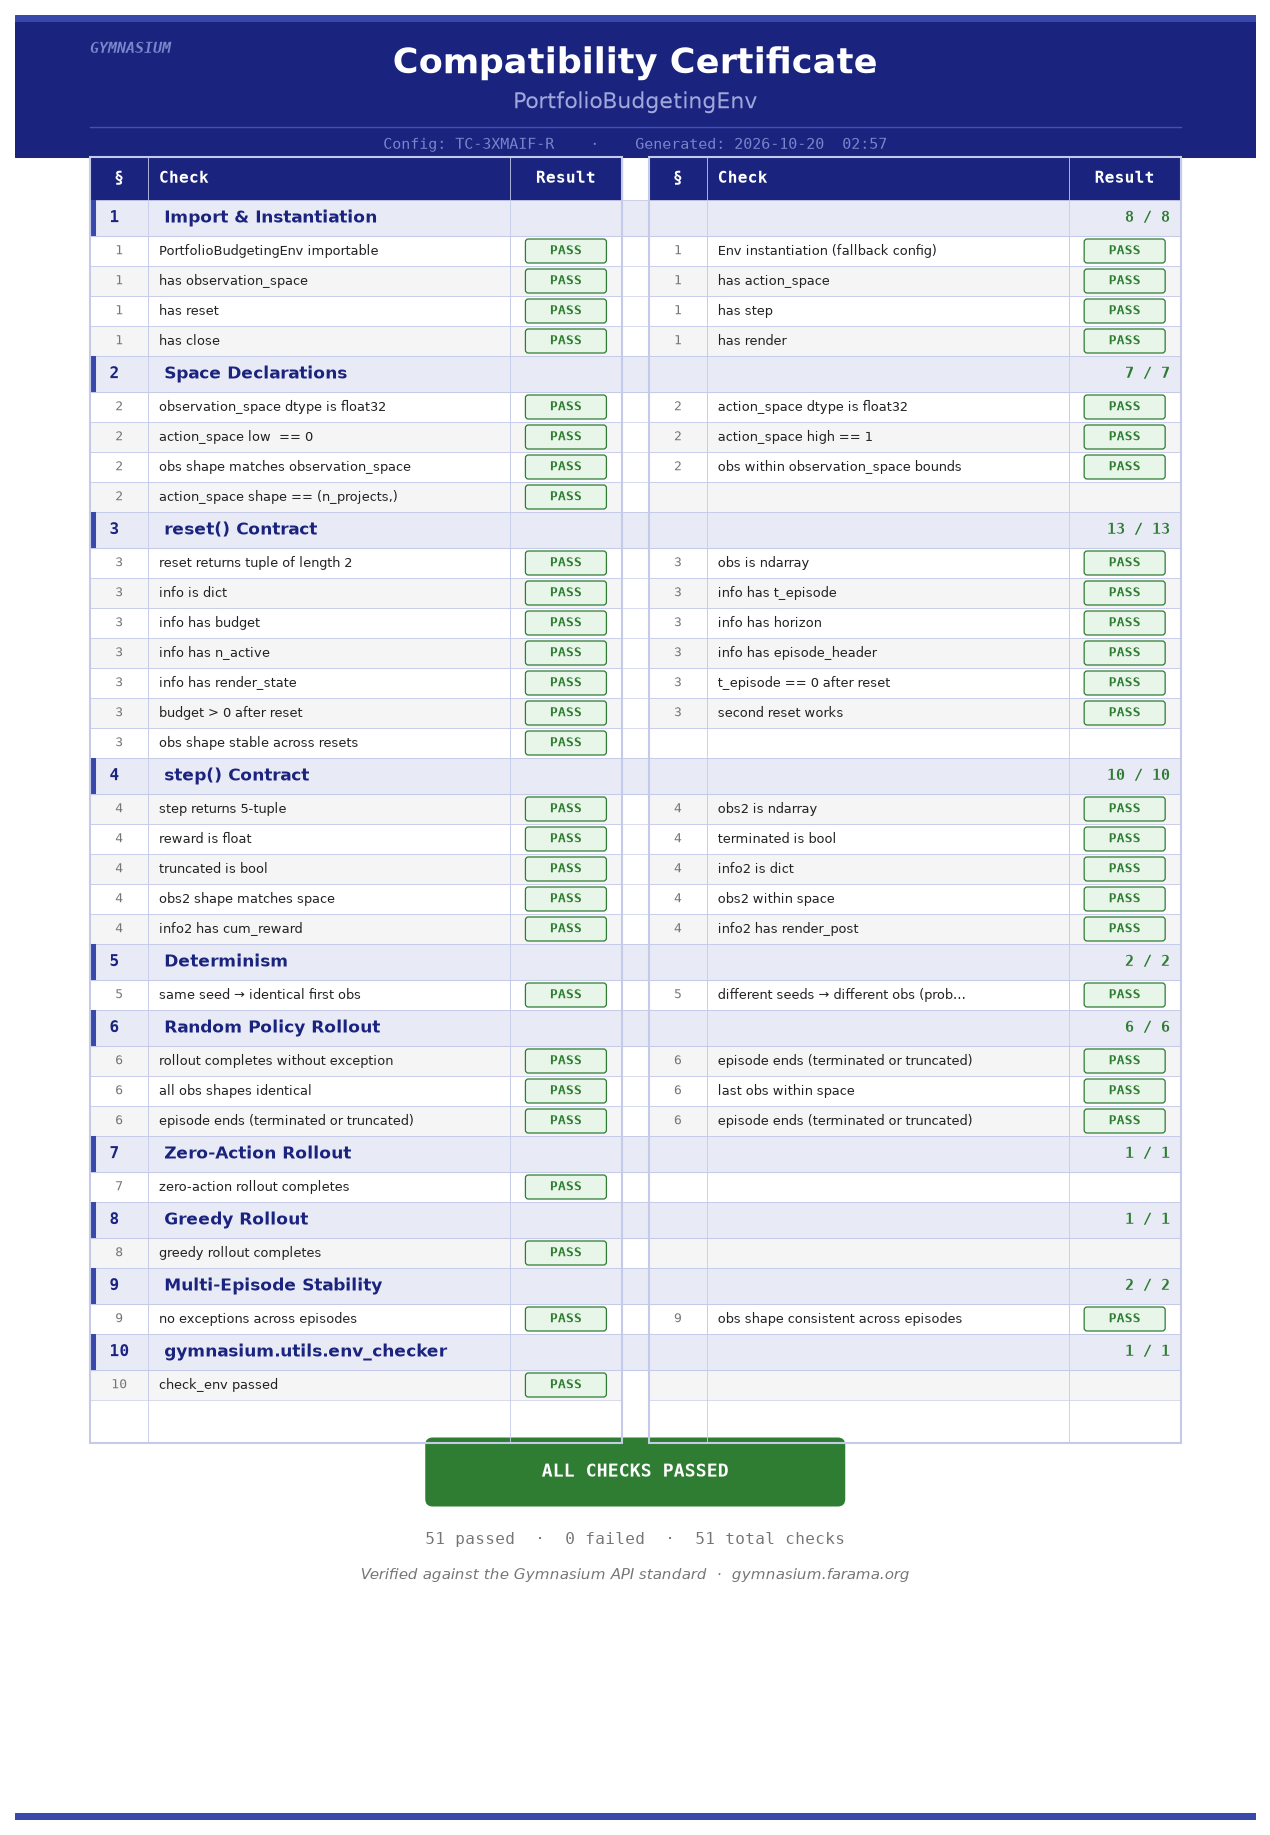
\includegraphics[width=0.82\textwidth]{figures/gym_certificate.png}
    \caption{Compatibility certificate generated by \texttt{tests/gym\_test.py}.
             All 51 checks pass; 0 failures.}
    \label{fig:gym_certificate}
\end{figure}